\chapter{\textbf{Технологический раздел}}

\hfill

В соответствии с выбранной задачей -- реализация микросервиса мессенджера. Необходимо выбрать средства реализации, создать модули и интерфейс, описать ограничения и порядок работы программы. 

\section{\textbf{Выбор технологий}}

Для выполнения проекта был выбран язык программирования C$\#$ \cite{csharp}. Язык является постоянно развивающимся, объектно-ориентированным. Он относится к семье языков с C-подобным синтаксисом, разрабатывался как язык программирования прикладного уровня для CLR (Common Language Runtime, общеязыковая исполняющая среда). 

Для разработки используется платформа ASP.NET Core \cite{aspnet}, предназначенная для создания различного рода веб-приложений: от небольших веб-сайтов до крупных веб-порталов и веб-сервисов. С помощью ASP.NET Core мы можем создавать кросс-платформенные приложения. Благодаря модульности фреймворка все необходимые компоненты веб-приложения могут загружаться как отдельные модули через пакетный менеджер Nuget.

Для доступа к данным используется технология Entity Framework Core \cite{ef}. EF Core является ORM-инструментом (object-relational mapping -- отображения данных на реальные объекты). То есть EF Core позволяет работать базами данных, но представляет собой более высокий уровень абстракции: EF Core позволяет абстрагироваться от самой базы данных и ее таблиц и работать с данными независимо от типа хранилища. 

Entity Framework Core поддерживает множество различных систем баз данных. Таким образом, мы можем через EF Core работать с любой СУБД, если для нее имеется нужный провайдер. Для работы с PostgeSQL в проект необходимо добавить через Nuget пакет Npgsql.EntityFrameworkCore.PostgreSQL. 

Для взаимодействия между клиентом и сервером используется архитектурный стиль REST \cite{rest}. API-интерфейс может считаться RESTful только в том случае, если соблюдены все требования. При создании микросервиса мессенджера были учтены данные требования, и поэтому веб-приложение является RESTful. 

Требования REST:
\begin{itemize}
\item модель клиент-сервер;
\item отсутствие состояния (сервис не хранит информацию о состоянии клиента);
\item кэширование;
\item единообразие интерфейса (идентификация ресурсов, манипуляция ресурсами через представление, «самоописываемые» сообщения);
\item многослойность сервера;
\item код по требованию (необязательно). 
\end{itemize}

\section{\textbf{Модель базы данных}}

На рисунке \ref{img:database} представлена модель базы данных. 

\begin{figure}[H]
	\centering
	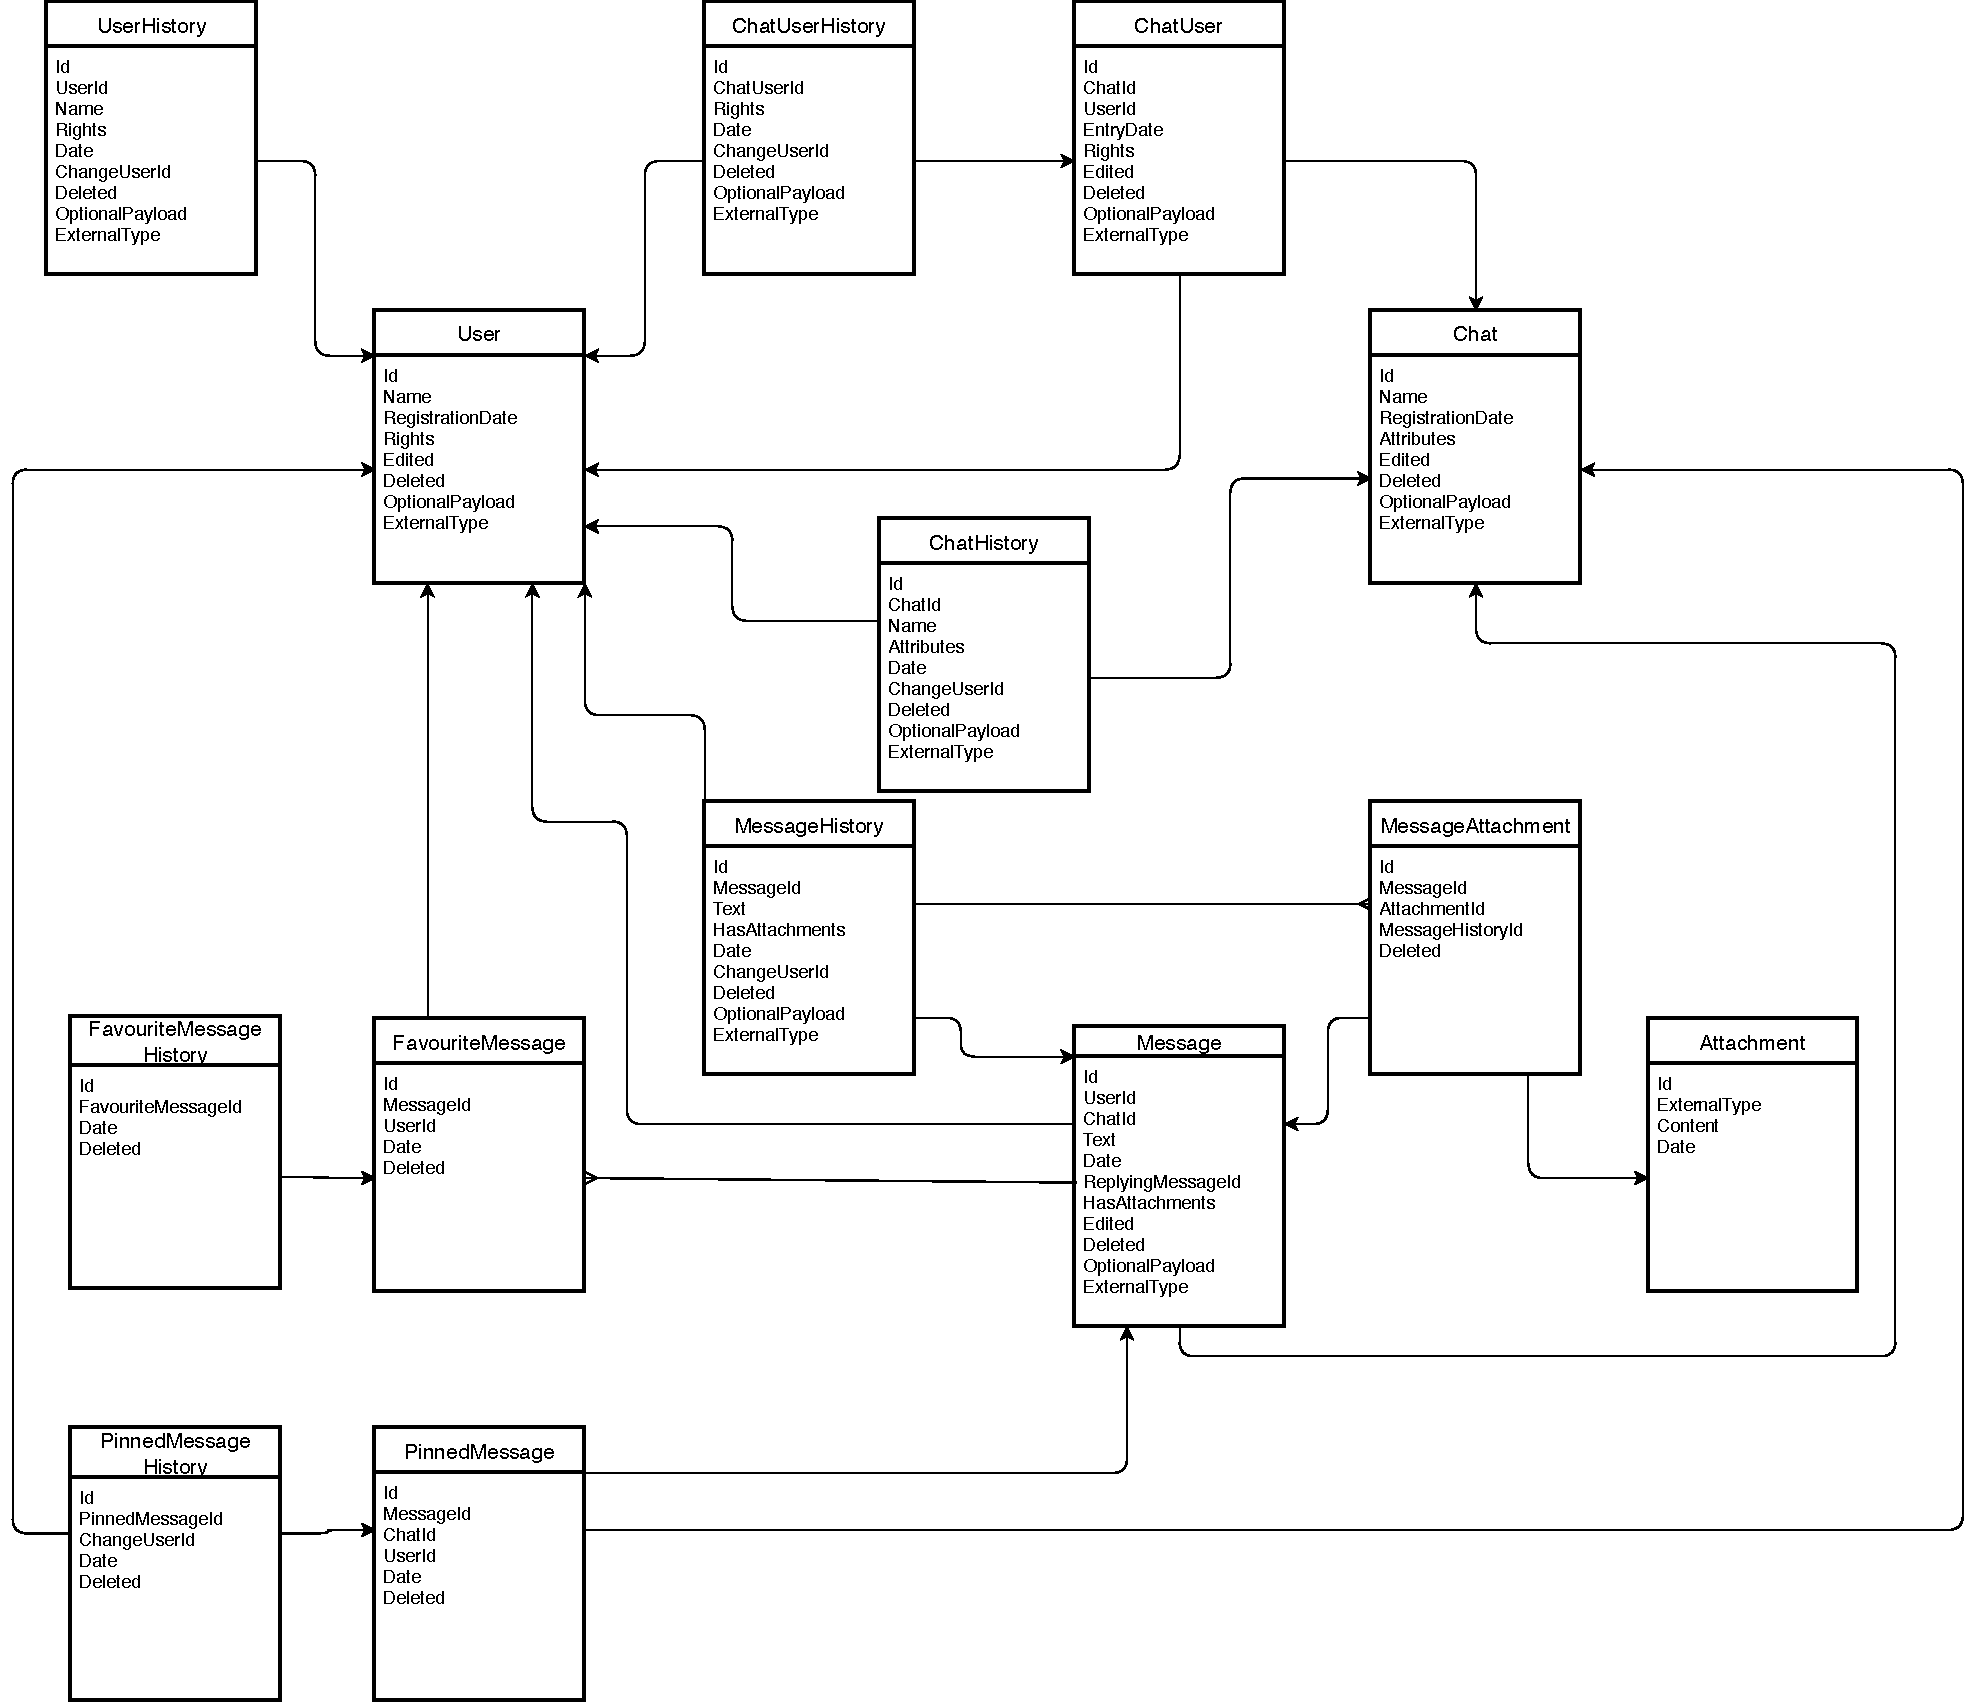
\includegraphics[scale=0.5]{database}
	\caption{Модель базы данных. }
	\label{img:database}
\end{figure}

\section{\textbf{UML-диаграммы классов }}

На рисунке \ref{img:databasemodels} представлена UML-диаграмма классов компонента ChatService.Database.Models. 

\begin{figure}[H]
	\centering
	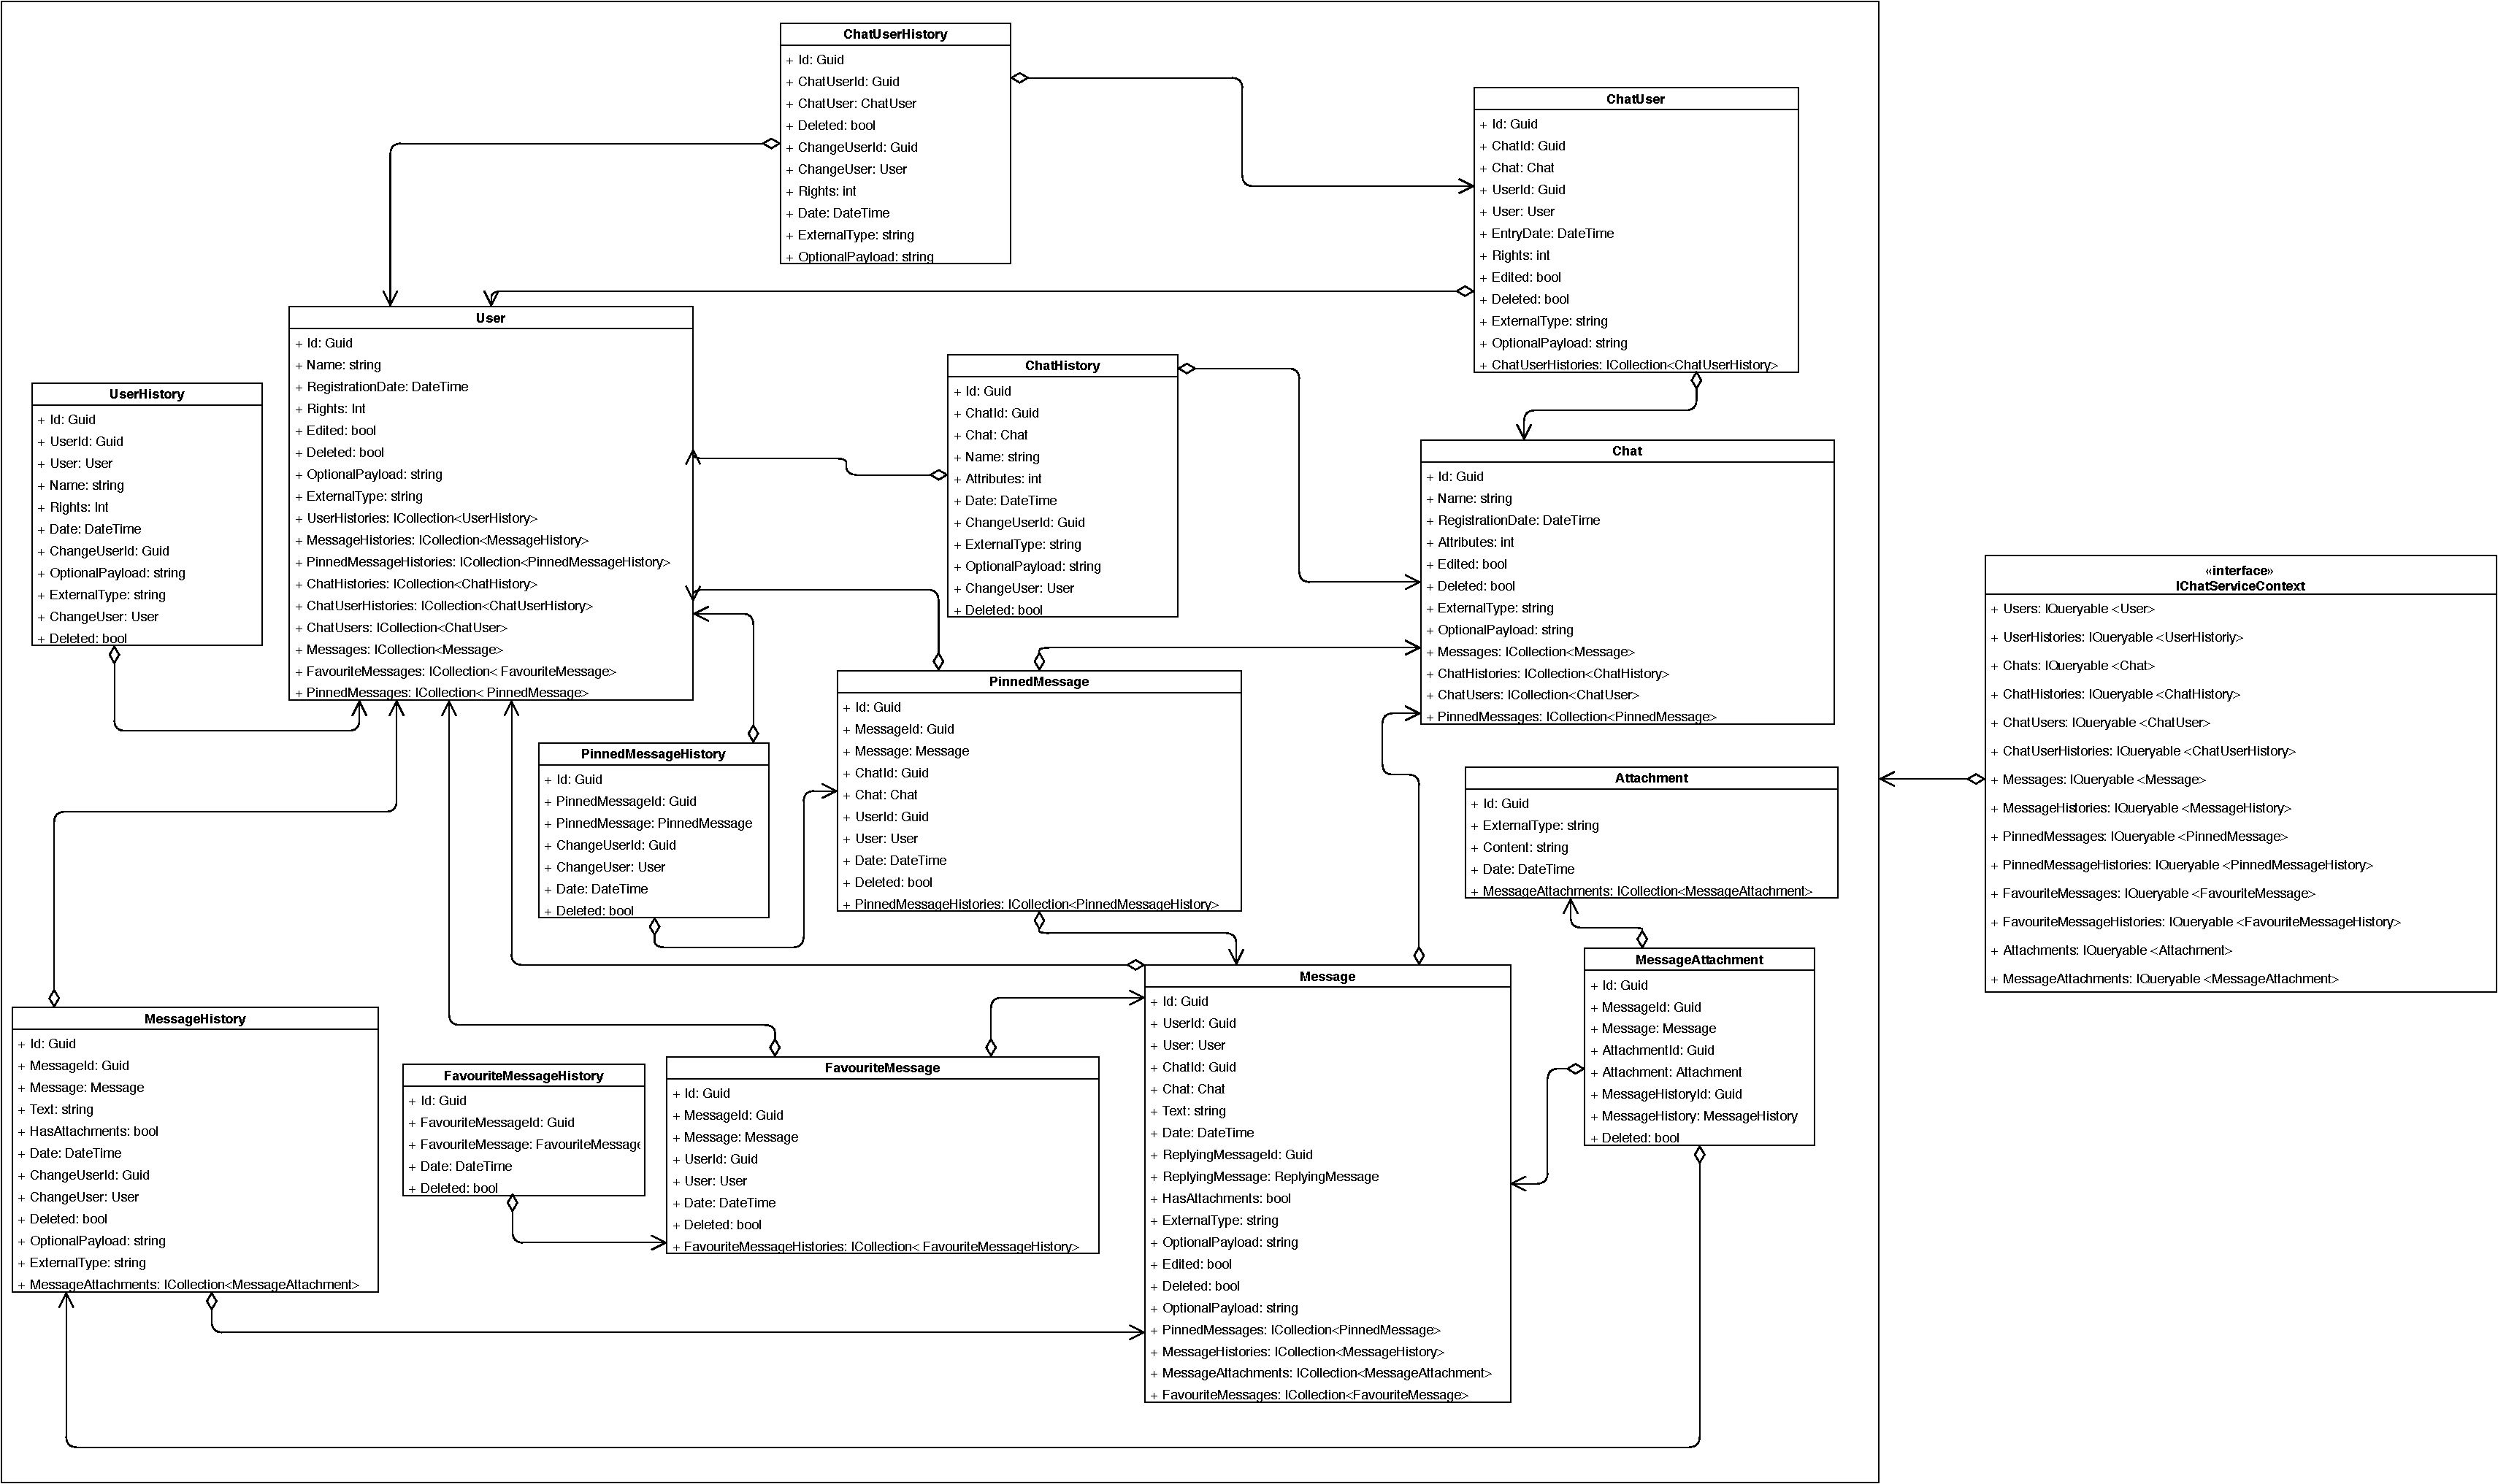
\includegraphics[scale=0.3]{databasemodels}
	\caption{UML-диаграмма классов компонента ChatService.Database.Models. }
	\label{img:databasemodels}
\end{figure}

На рисунке \ref{img:npgsqlcontext} представлена UML-диаграмма классов компонента ChatService.Database.NpgsqlContext. 

\begin{figure}[H]
	\centering
	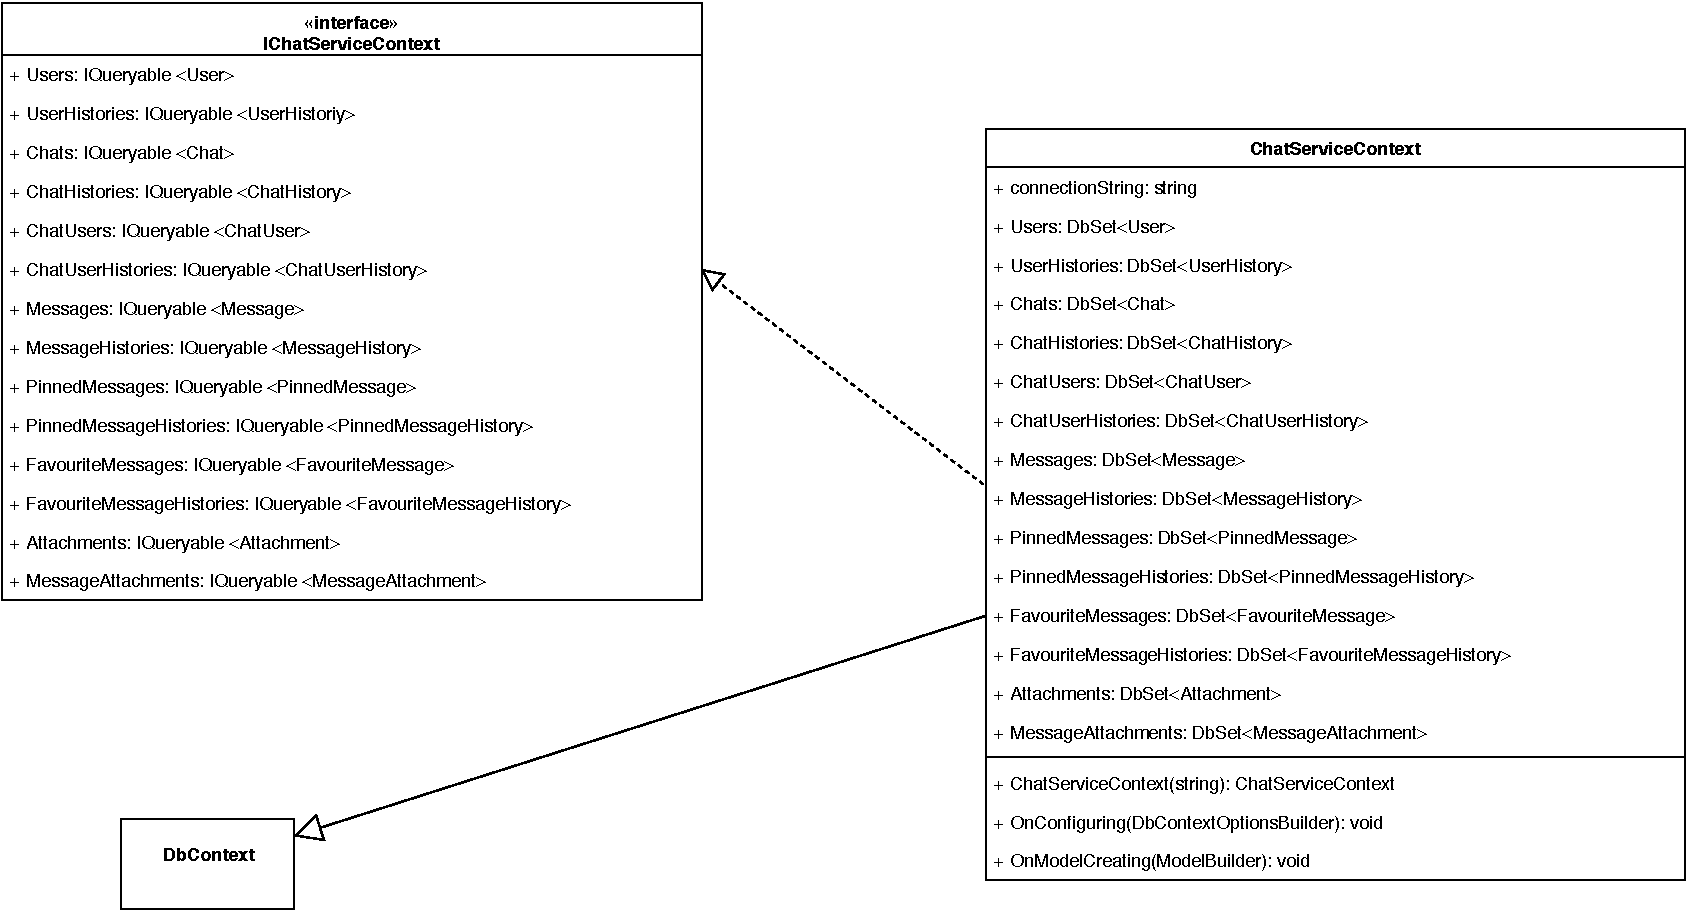
\includegraphics[scale=0.60]{npgsqlcontext}
	\caption{UML-диаграмма классов компонента ChatService.Database.NpgsqlContext. }
	\label{img:npgsqlcontext}
\end{figure}

На рисунке \ref{img:core} представлена UML-диаграмма классов компонента ChatService.Core. 

\begin{figure}[H]
	\centering
	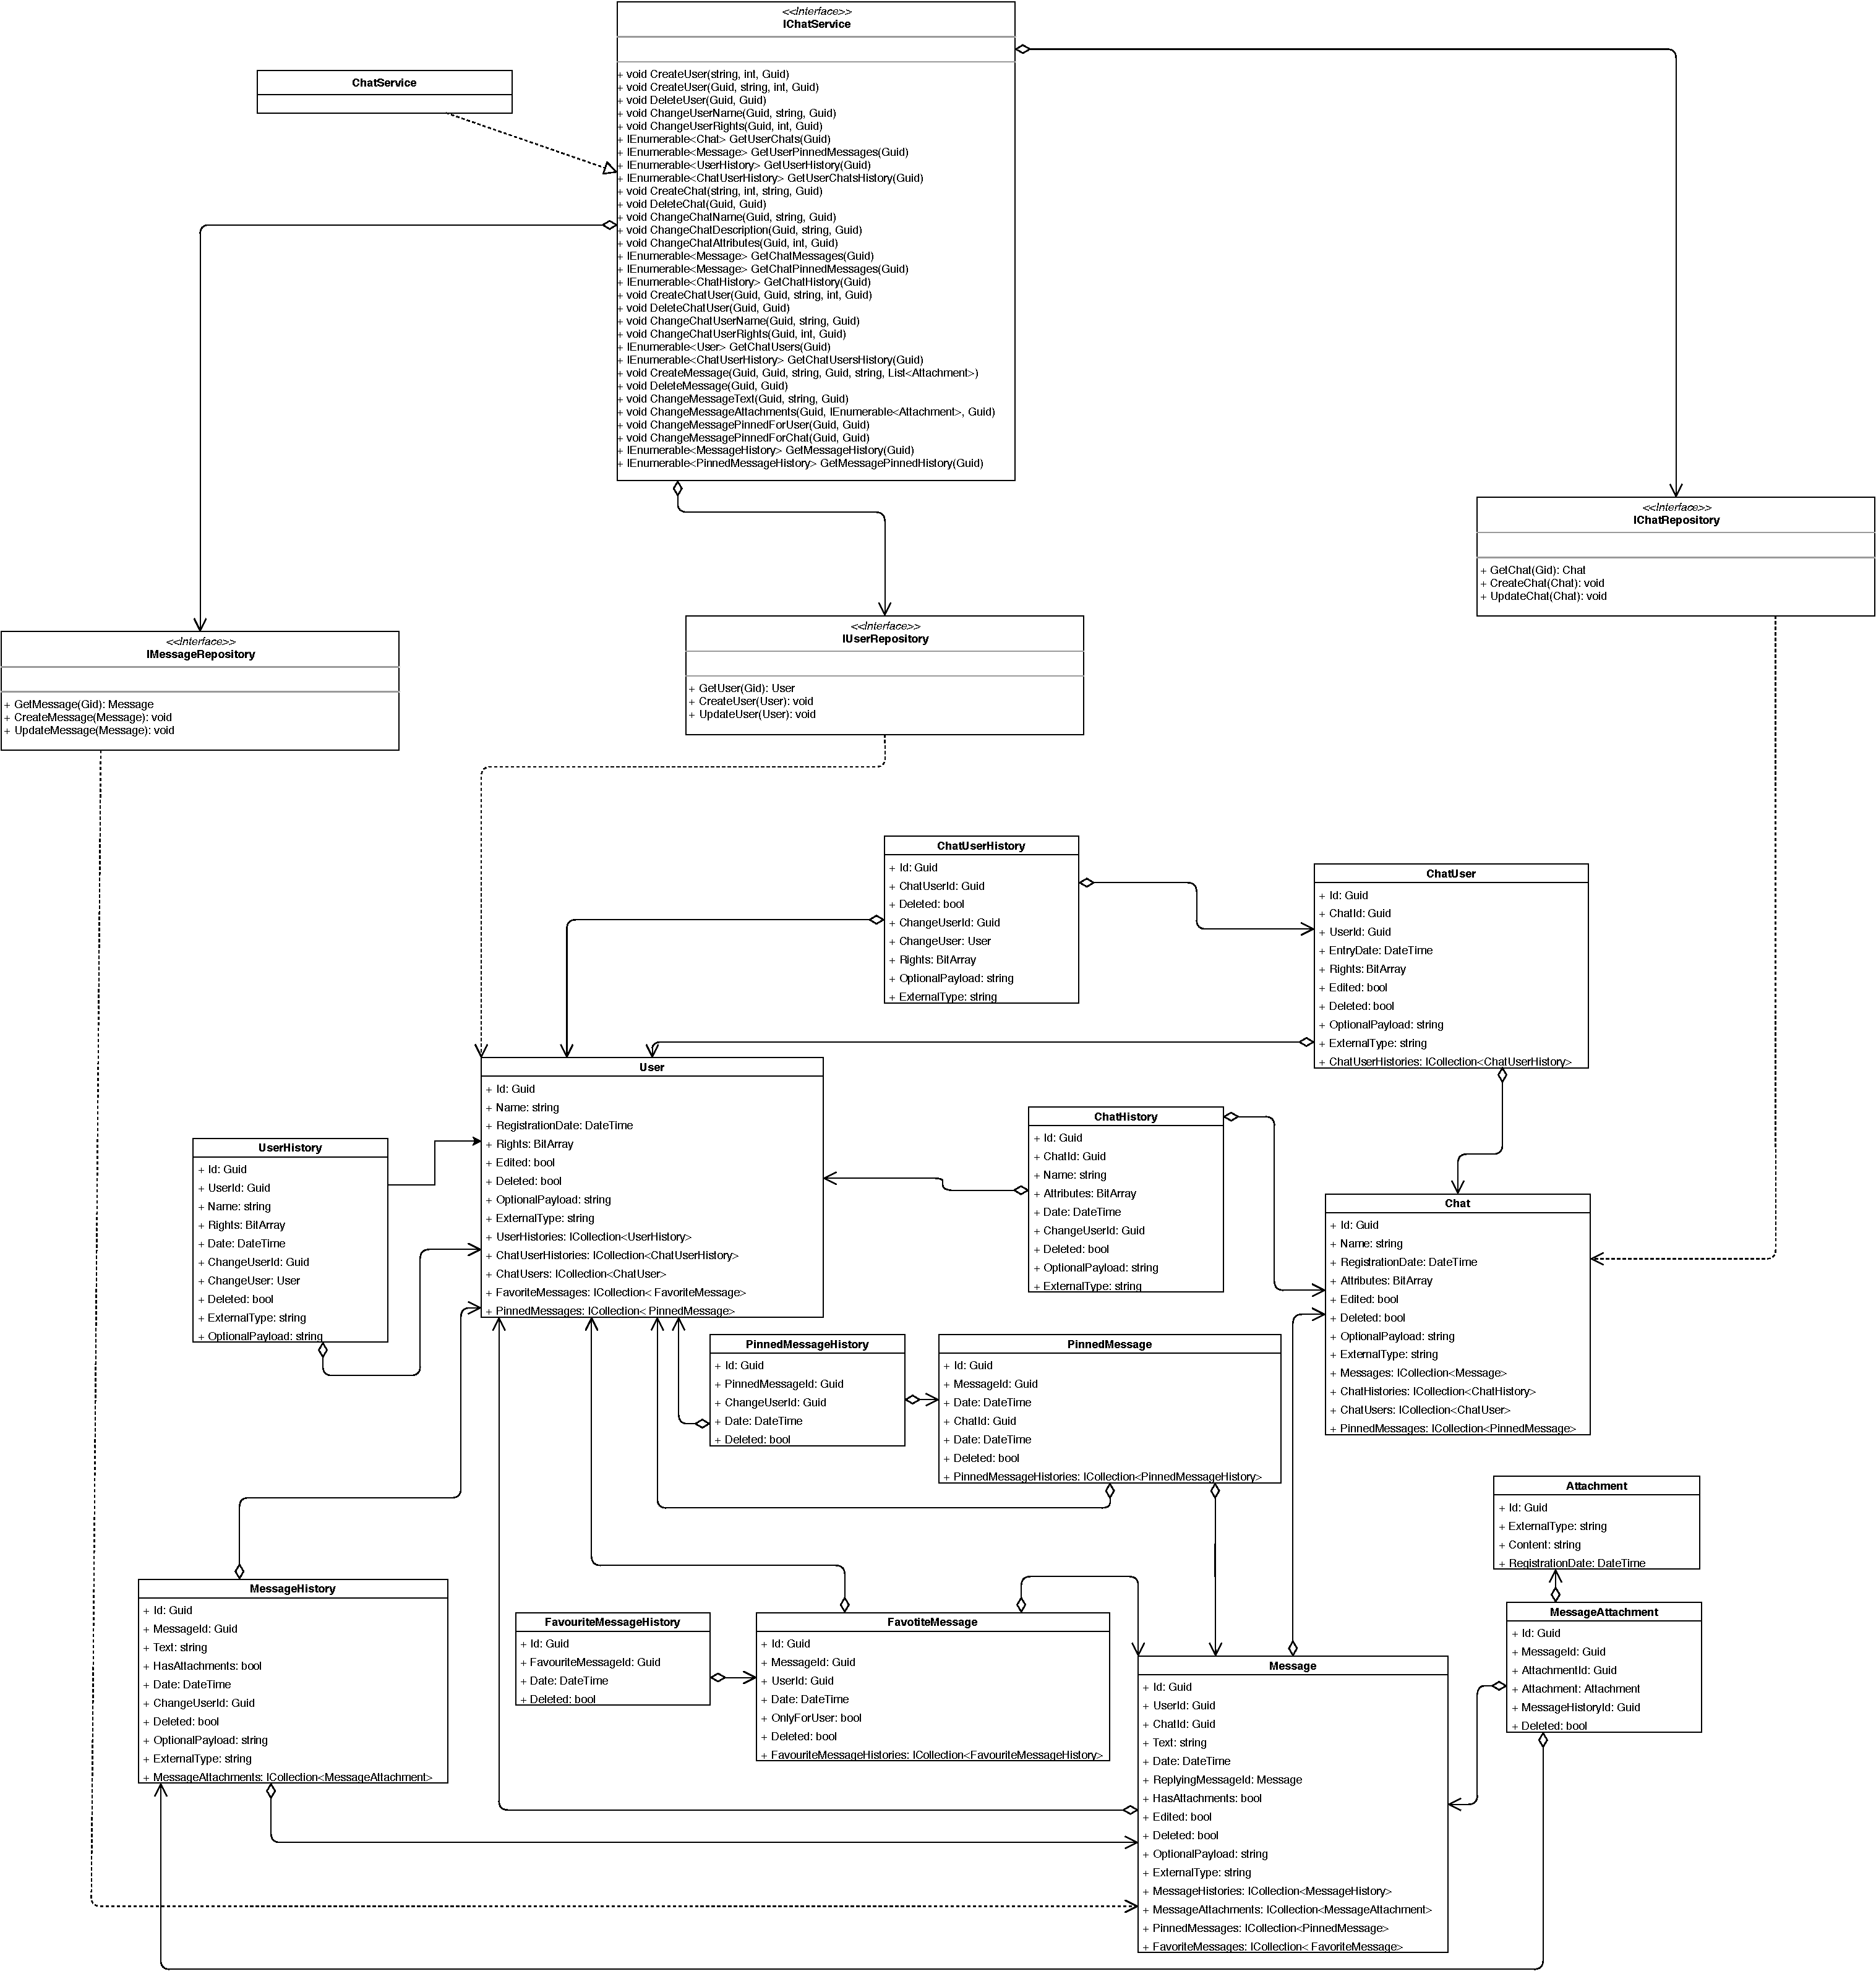
\includegraphics[scale=0.35]{core}
	\caption{UML-диаграмма классов компонента ChatService.Core. }
	\label{img:core}
\end{figure}

\textbf{Описание методов данного компонента:}
\begin{itemize}
\item void CreateUser(string name, int rights, Guid changeUserId) - добавление пользователя
\item void CreateUser(Guid userId, string name, int rights, Guid changeUserId) - добавление пользователя
\item void DeleteUser(Guid userId, Guid changeUserId) - удаление пользователя
\item void ChangeUserName(Guid userId, string newName, Guid changeUserId) - изменение имени пользователя
\item void ChangeUserRights(Guid userId, int newRights, Guid changeUserId) - изменение прав пользователя
\item IEnumerable<Chat> GetUserChats(Guid userId) - получение списка чатов пользователя
\item IEnumerable<Message> GetUserPinnedMessages(Guid userId) - получение списка избранных сообщений пользователя
\item IEnumerable<UserHistory> GetUserHistory(Guid userId) - получение всей истории пользователя
\item IEnumerable<ChatUserHistory> GetUserChatsHistory(Guid userId) - получение истории чатов пользователя
\item void CreateChat(string name, int attributes, string desciption, Guid changeUserId) - добавление чата
\item void DeleteChat(Guid chatId, Guid changeUserId) - удаление чата
\item void ChangeChatName(Guid chatId, string newName, Guid changeUserId) - изменение имени чата
\item void ChangeChatDescription(Guid chatId, string newDescription, Guid changeUserId) - изменение описания чата
\item void ChangeChatAttributes(Guid chatId, int newAttributes, Guid changeUserId) - изменение аттрибутов чата
\item IEnumerable<Message> GetChatMessages(Guid chatId) - получение сообщений чата
\item IEnumerable<Message> GetChatPinnedMessages(Guid chatId) - получение припиненных сообщений чата
\item IEnumerable<ChatHistory> GetChatHistory(Guid chatId) - получение истории чата
\item void CreateChatUser(Guid chatId, Guid userId, string name, int rights, Guid changeUserId) - добавление пользователя в чат
\item void DeleteChatUser(Guid chatUserId, Guid changeUserId) - удаление пользователя из чата
\item void ChangeChatUserName(Guid chatUserId, string newName, Guid changeUserId) - изменение имени пользователя чата
\item void ChangeChatUserRights(Guid chatUserId, int rights, Guid changeUserId) - изменение прав пользователя чата
\item IEnumerable<User> GetChatUsers(Guid chatId) - получение пользователей чата
\item IEnumerable<ChatUserHistory> GetChatUsersHistory(Guid chatId) - получение истории пользователей чата
\item void CreateMessage(Guid userId, Guid chatId, string text, Guid replyingMessageId, string type, List<Attachment> messageAttachments) - добавление сообщения
\item void DeleteMessage(Guid messageId, Guid changeUserId) - удаление сообщения
\item void ChangeMessageText(Guid messageId, string newText, Guid changeUserId) - изменение текста сообщения
\item void ChangeMessageAttachments(Guid messageId, IEnumerable<Attachment> newMessageAttchments, Guid changeUserId) - изменение вложений сообщения
\item void ChangeMessagePinnedForUser(Guid userId, Guid changeUserId) - припинивание/отпинивание сообщения для пользователя
\item void ChangeMessagePinnedForChat(Guid userId, Guid changeUserId) - припинивание/отпинивание сообщения для чата
\item IEnumerable<MessageHistory> GetMessageHistory(Guid messageId) - получение истории сообщения
\item IEnumerable<PinnedMessageHistory> GetMessagePinnedHistory(Guid messageId) - получение истории припинивания сообщения
\end{itemize}

\section{\textbf{Тестовое клиентское приложение }}

Реализовано с помощью 

Запуск приложения представлен на рисунке \ref{img:init}. 

\begin{figure}[H]
	\centering
	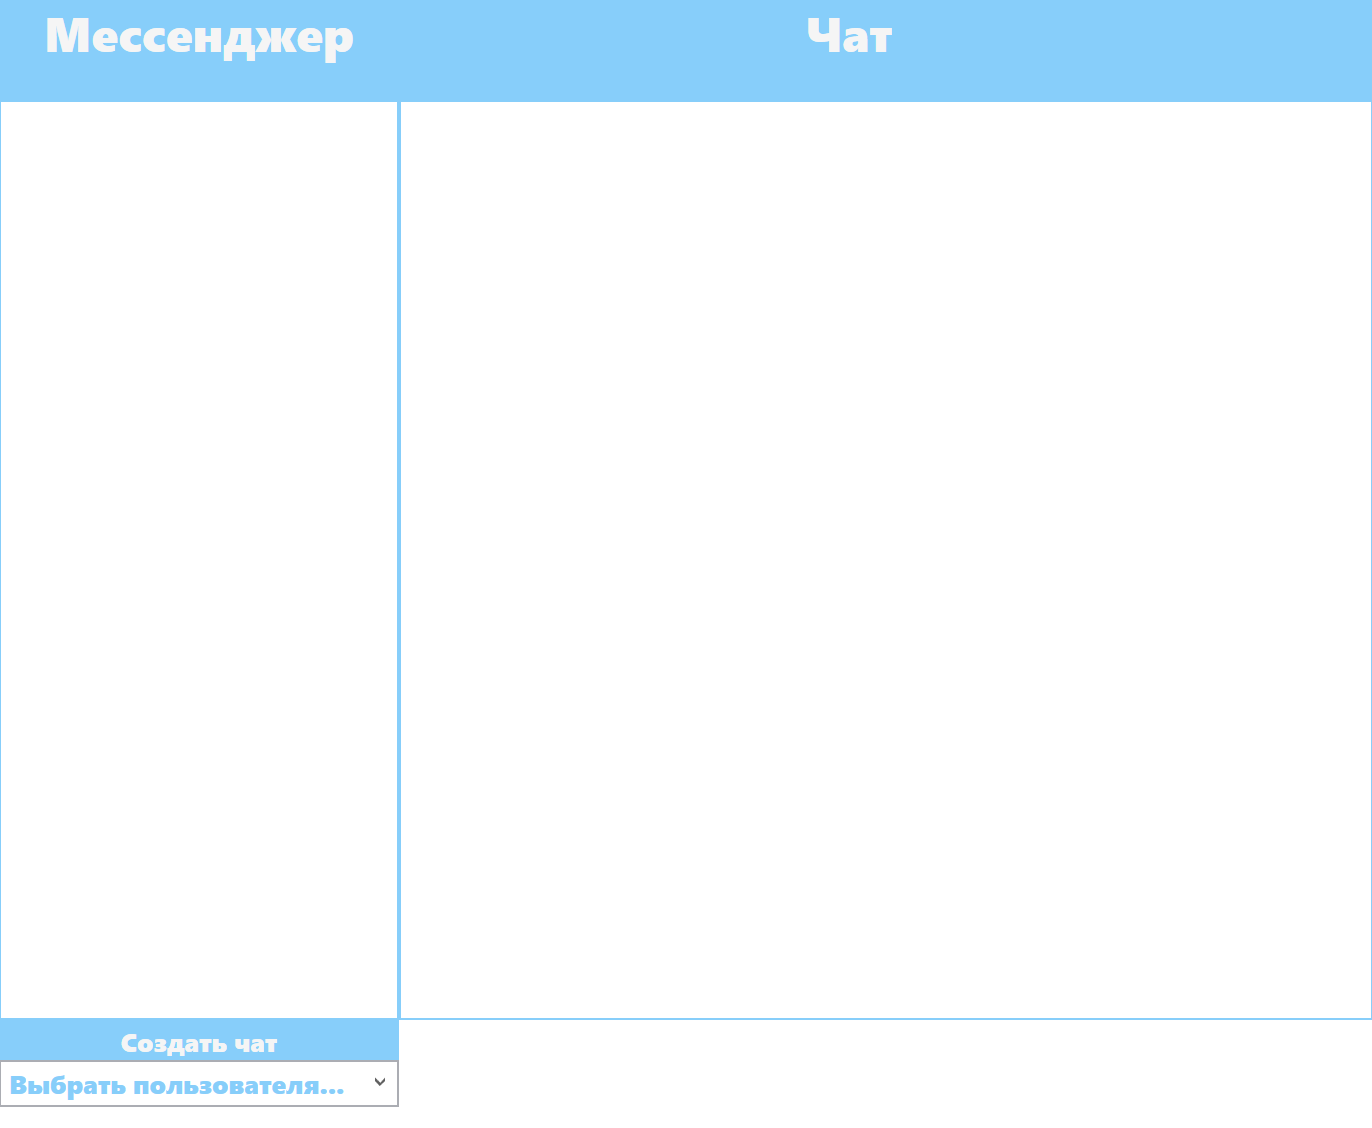
\includegraphics[scale=0.7]{init}
	\caption{Начальный экран приложения.  }
	\label{img:init}
\end{figure}

Далее можно выбрать текущего пользователя, от имени которого будут происходить дальнейшие действия, рисунок \ref{img:users}. 

\begin{figure}[H]
	\centering
	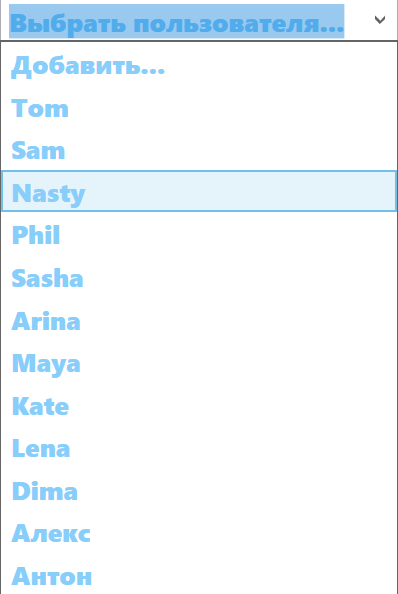
\includegraphics[scale=1]{users}
	\caption{Выбор пользователя.  }
	\label{img:users}
\end{figure}

Далее можно выбрать чат, рисунок \ref{img:messenger}.

Сообщения чата обновляются каждую секунду. Отправить сообщение можно либо по нажатию на кнопку, либо по нажатию на клавишу "Enter". Отправка пустого сообщения невозможна. 

\begin{figure}[H]
	\centering
	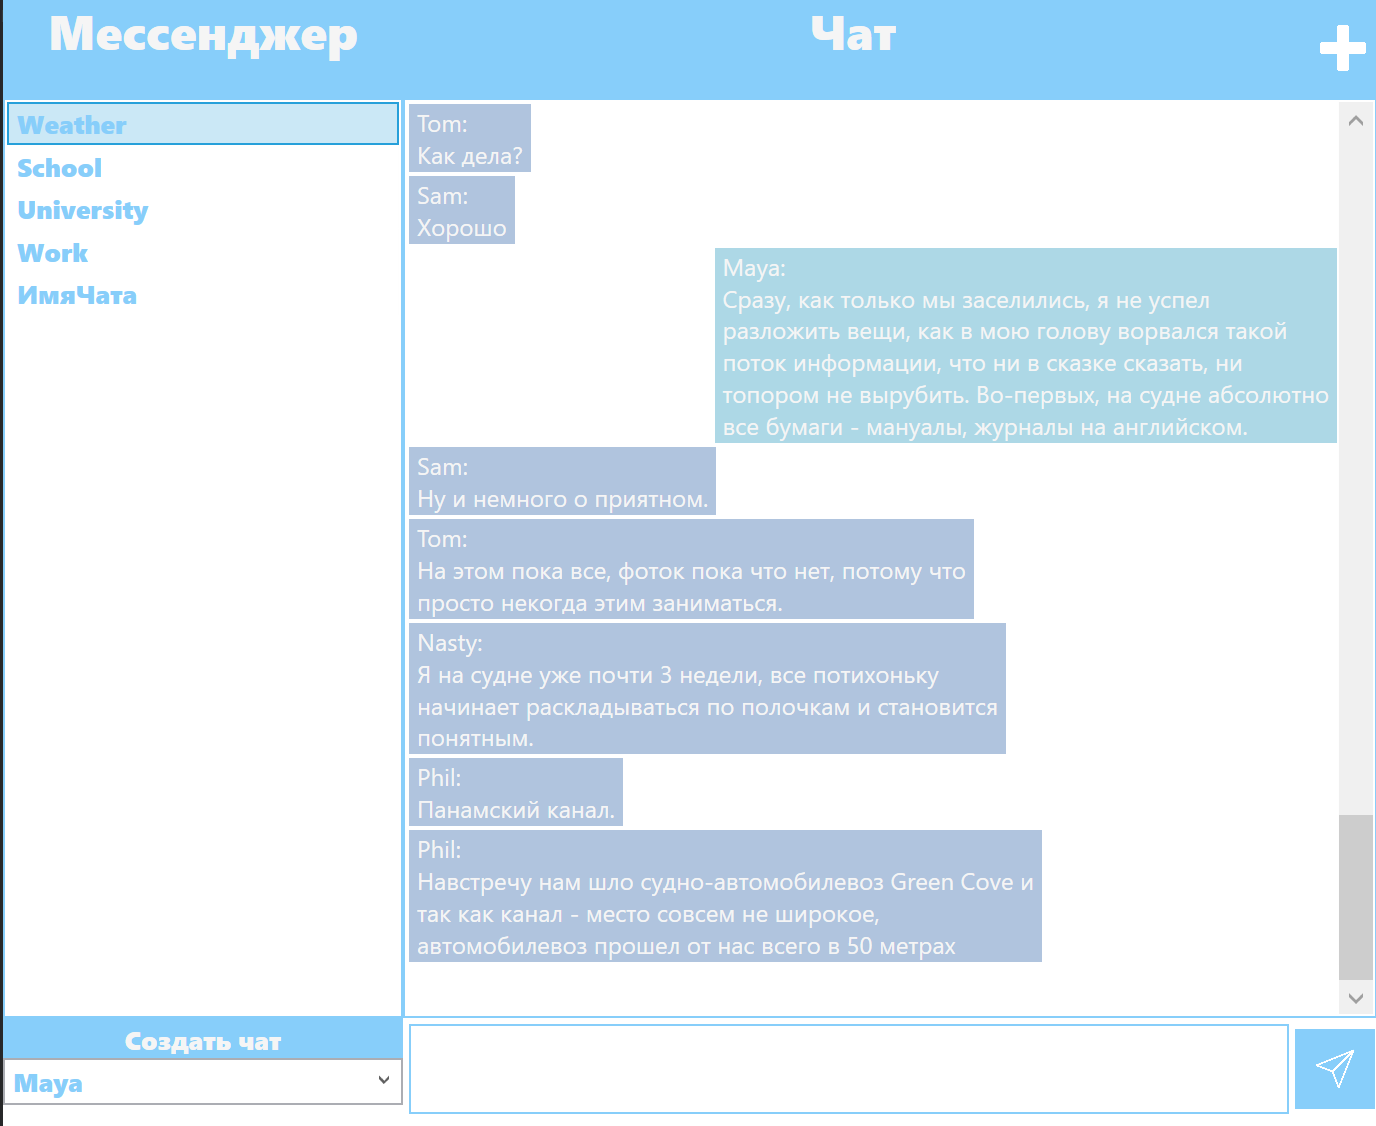
\includegraphics[scale=0.7]{messenger}
	\caption{Выбор чата, отображение сообщений.  }
	\label{img:messenger}
\end{figure}

Есть возможность из интерфейса создать новый чат (\ref{img:addchat}), нового пользователя \ref{img:adduser} или добавить пользователей (одного или нескольких) в уже существующий чат \ref{img:addchatuser}. 

\begin{figure}[H]
	\centering
	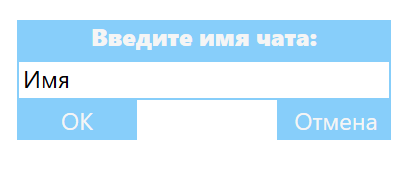
\includegraphics[scale=1]{addchat}
	\caption{Создание чата.  }
	\label{img:addchat}
\end{figure}

\begin{figure}[H]
	\centering
	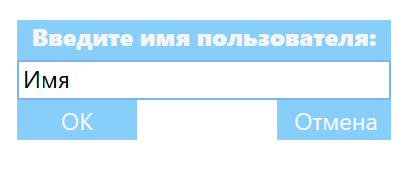
\includegraphics[scale=1]{adduser}
	\caption{Создание пользователя.  }
	\label{img:adduser}
\end{figure}

\begin{figure}[H]
	\centering
	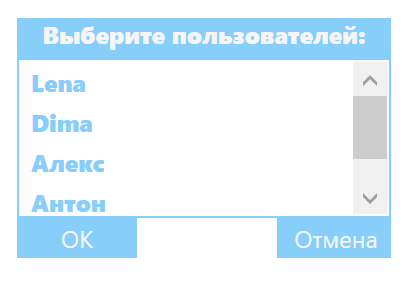
\includegraphics[scale=1]{addchatuser}
	\caption{Добавление пользователя/пользователей чат.  }
	\label{img:addchatuser}
\end{figure}

\section{\textbf{Администрирование БД}}

С использованием pgAdmin (программное обеспечение, предоставляющее графический интерфейс для работы с базой данных) было проверено корректное создание базы данных с необходимыми ключами. 

На рисунке \ref{img:tables} показано существование таблицы в БД. 

\begin{figure}[H]
	\centering
	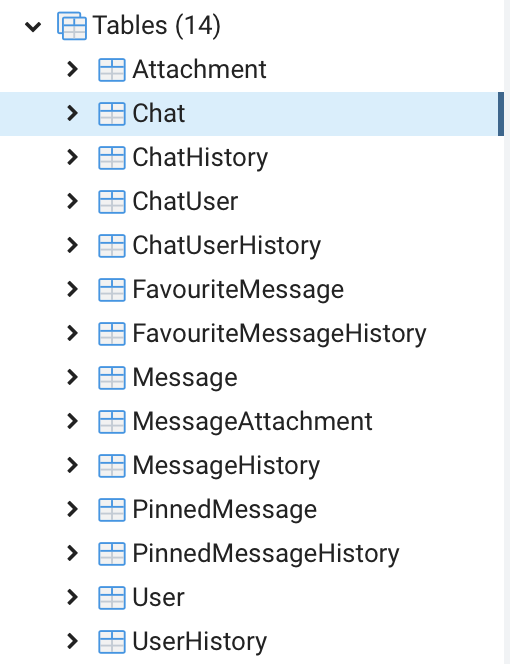
\includegraphics[scale=1]{tables}
	\caption{Таблицы базы данных.  }
	\label{img:tables}
\end{figure}

На рисунке \ref{img:chattable} показан пример корректности ключей для таблицы чатов.  

\begin{figure}[H]
	\centering
	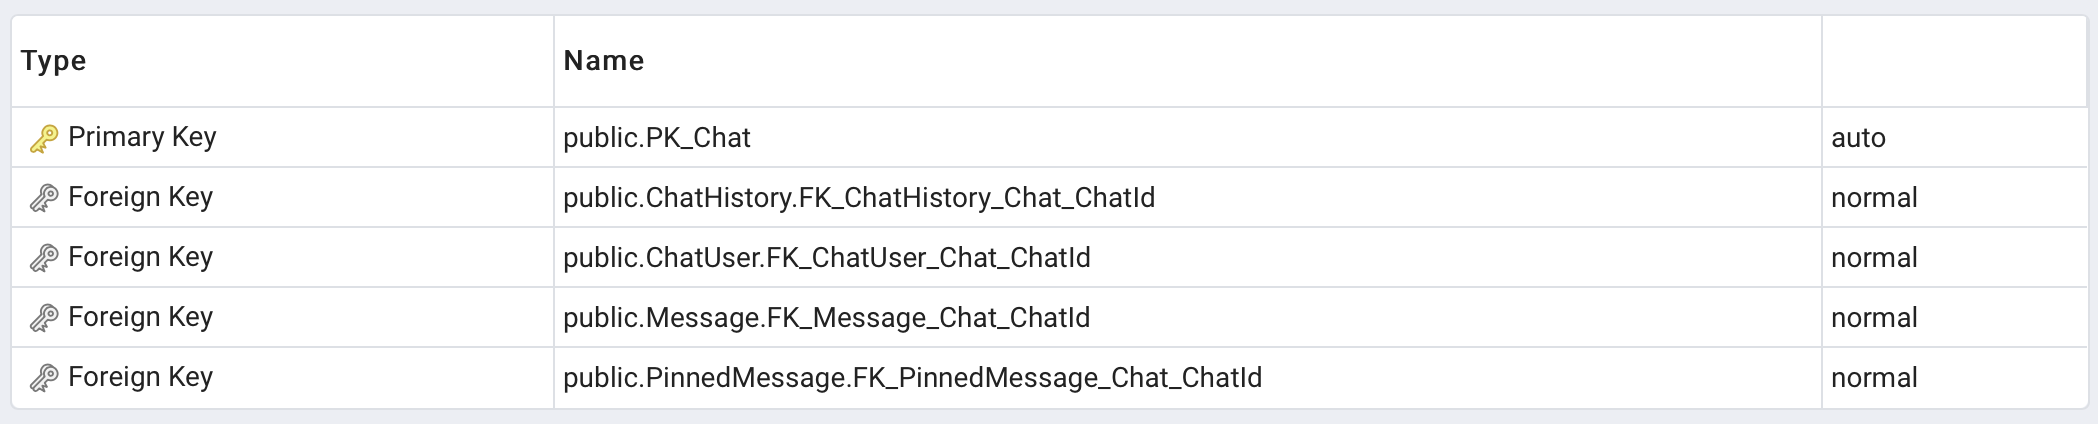
\includegraphics[scale=0.45]{chattable}
	\caption{Ключи таблицы чатов. }
	\label{img:chattable}
\end{figure}


\section{\textbf{Вывод}}

Реализовано спроектированное ПО, представлены результаты. 
